\documentclass[mathserif]{beamer}
\usetheme{Luebeck}
%\usepackage[francais]{babel}
\usepackage[utf8]{inputenc} % Uses the utf8 input encoding
\usepackage[T1]{fontenc} % Use 8-bit encoding that has 256 glyphs

\usepackage[nomath]{kpfonts}
\usepackage{eulervm}
%\usepackage{default}

\usepackage{amsthm}
\usepackage{amssymb}
\usepackage{xparse}
\usepackage{thmtools}
\usepackage{stackrel}

%shortcuts
\newcommand{\R}{\mathbb{R}}
\newcommand{\C}{\mathbb{C}}
\newcommand{\Z}{\mathbb{Z}}
\newcommand{\N}{\mathbb{N}}
\newcommand{\fii}{\varphi}
\newcommand{\dd}{\mathrm{d}}
\newcommand{\CP}{\mathbb{CP}}
\renewcommand{\S}{\mathbb{S}}
\DeclareMathOperator{\Sp}{Sp}
\DeclareMathOperator{\tr}{tr}
\DeclareMathOperator{\dist}{dist}

% theorems configuration

\makeatletter
\newtheoremstyle{indented}
{7pt} %vertical space before
{7pt} % vertical space after
{} %{\addtolength{\@totalleftmargin}{2.5em}
	%\addtolength{\linewidth}{-3.5em}
	%\parshape 1 3.5em \linewidth} %body font
{1.5em} %indent
{\bfseries} %header font
{.} %punctuation
{.5em} %horizontal space after header
{} %header specification

\theoremstyle{definition}

\newtheorem{defn}{Définition}[section]

\theoremstyle{plain}
%\newtheorem*{theorem*}{Theorem}

\newtheorem{thm}{Théorème}

\renewcommand{\thetheorem}{\Alph{theorem}}
\newenvironment{preuve}{
	\noindent \textbf{Proof. }}{\hfill $\square$\medskip\par}

\newtheorem{exemple}[defn]{Example}
\newtheorem{prop}[defn]{Proposition}
\newtheorem{corr}[defn]{Corollary}
\newtheorem{por}[defn]{Porisme}
\newtheorem{ex}[defn]{Example}
\newtheorem{lem}[defn]{Lemma}
\newtheorem{conj}{Conjecture}
\newtheorem{ax}{Axiom}  %Axioms have their own numerotation

\theoremstyle{definition}
\newtheorem{rem}[defn]{Remark} %remarks are not indented
\newtheorem{rems}[defn]{Remarks}

%--------------
% Mise en page mathématique
%--------------
\addtolength{\jot}{.2em}


\title[Eigenfunctions concentration for Toeplitz operators]{Concentration of
  eigenfunctions for semiclassical Toeplitz operators}
\author[Alix Deleporte]{Alix Deleporte\\Advisor : Nalini Anantharaman}
\institute[IRMA]{Institut de Recherche Mathématique
  Avancée\\Université de Strasbourg}

\AtBeginSection
{
	\begin{frame}
		\frametitle{Plan}
		\tableofcontents[currentsection]
	\end{frame}
	
}

\newcommand{\spline}{\hline}
\renewcommand{\arraystretch}{1.3}
\begin{document}
\begin{frame}
	\titlepage
\end{frame}

\section{Toeplitz opreators}
\subsection{Toeplitz operators on $\C^n$}
\begin{frame}
  \frametitle{Bargmann spaces}
  \begin{itemize}
  \item Original idea: express Quantum Mechanics directly in phase
    space.
  \uncover<2->{\item The standard $L^2(\R^n)$ is replaced with the \emph{Bargmann
      space}, with parameter $N>0$:
$$B_N=L^2(\C^n)\cap\left\{e^{-\frac N2 |\cdot|^2}f,\,f\text{ is
  holomorphic on $\C^n$}\right\}.$$}\vspace{-2em}
  \uncover<3>{\item This is a closed subspace of $L^2(\C^n)$, with reproducing
    kernel
$$\Pi_N(x,y)=\left(\frac N{\pi}\right)^n\exp\left(-\cfrac N2
  |x-y|^2+iN\Im(x\cdot \overline{y})\right).$$}
  \end{itemize}
\vspace{-1em}
\small{[1] Bargmann, V. Comm. Pure Appl. Math. 14, no. 3 (1961): 187–214.}

\end{frame}

\begin{frame}
  \frametitle{Szeg\H{o} kernel}
  Hilbert basis indexed by $\N^{n}$:

$$e_{\nu}=\uncover<2->{\cfrac{N^{|\nu|}}{\nu_1!\nu_2!\ldots\nu_n!}}\,z^{\nu}e^{-\frac{N|z|^2}{2}}.$$

\uncover<3>{From there one recovers $\Pi_N$ with
$$\Pi_N(x,y)=\sum_{\nu\in \N^n} e_{\nu}(x)\overline{e_{\nu}}(y).$$

The Szeg\H{o} kernel decays exponentially fast away from the diagonal.
}
\end{frame}

\begin{frame}
  \frametitle{Toeplitz quantization}
  Let $f\in C^{\infty}(\C^n,\C)$ bounded. The Toeplitz operator associated
  with $f$ is the bounded operator
\begin{center}
\begin{array}{rcl}
 		T_N(f):B_N(\C^n)&\mapsto & B_N(\C^n)\\
		u& \mapsto& \uncover<2->{\Pi_N(}fu\uncover<2->{)}.
 		\end{array}
\end{center}

\uncover<3->{If $f$ has polynomial growth then $T_N(f)$ is an unbounded operator
with dense domain.}
\uncover<4>{\begin{itemize}
\item If $f$ is real-valued then $T_N(f)$ is ess. self-adjoint.
\item If moreover $f\geq 0$ then $T_N(f)\geq 0$.
\end{itemize}}
\end{frame}

\begin{frame}
  \frametitle{Composition of Toeplitz operators}
  \begin{itemize}
  \item Recipe: \[T_N(z\mapsto \overline{z}^{\alpha}z^{\beta})=N^{-|\alpha|}\partial^{\alpha}z^{\beta}.\]

\uncover<2->{\item The Toepliz quantization is \emph{anti-Wick}: if $f$ is
  anti-holomorphic and $h$ is holomorphic then
\[T_N(fgh)=T_N(f)T_N(g)T_N(h).\]}
\uncover<3>{\vspace{-1.5em}\item More generally, composition yields a formal series:
\[T_N(f)T_N(g)=T_N\left(fg+N^{-1}C_1(f,g)+N^{-2}C_2(f,g)+\cdots\right).\]

$C_j$ is a bidifferential operator of total order $2j$.}
\end{itemize}
\end{frame}

\begin{frame}
  \frametitle{Toeplitz operators versus $\Psi$DOs}
  \begin{itemize}
  \item The Bargmann transform $\mathcal{B}_N$ conjugates $B_N$ and
    $L^2(\R^n)$.
  \uncover<2->{\item It is related to the FBI
    transform.}
  \uncover<3->{
  \item With $g_N=(N/\pi)^ne^{-N|z|^2}$ one has
    \[
      \mathcal{B}_N^{-1}T_N(f)\mathcal{B}_N=Op_W^{N^{-1}}(f*g_N).
    \]\vspace{-2em}}
\uncover<4->{\item Formal equivalence between Toeplitz and $\Psi$DO
  calculus.}
\uncover<5>{\item Toeplitz quantization is formulated directly in phase space!}
  \end{itemize}
\end{frame}

\subsection{Toeplitz operators on compact manifolds}
\begin{frame}
  \frametitle{Hardy spaces and Szeg\H{o} kernel}
  \begin{itemize}
  \item Geometrical setting: compact K\"ahler manifold $M$.\\
    \begin{minipage}{0.37\linewidth}\begin{itemize}
    \item Symplectic form
    \item Complex structure
    \end{itemize}
\end{minipage}
\uncover<2->{\begin{minipage}{0.52\linewidth}

$\biggl\}$ Compatibility condition
\end{minipage}}
\uncover<3->{\item Complex line bundle $L\to M$ with curvature $-i\omega$.}
\uncover<4->{\item Hardy space $H_N(M,L)$ of holomorphic sections of $L^{\otimes N}$.}
\uncover<5->{\item Szeg\H{o} projector $S_N:L^2(M,L^{\otimes N})\to H_N(M,L).$}
  \end{itemize}
\uncover<6>{The spaces $H_N(M,L)$ are finite-dimensional in that case. The
line bundles $L^{\otimes N}$ correspond to the weights $e^{-\frac N2
  |\cdot|^2}$ in the flat case.}
\vspace{1em}

\small{[2] Woodhouse, N. Geometric Quantization. Oxford University Press, 1997.}
\end{frame}

\begin{frame}
  \frametitle{Algebra of Toeplitz operators}
  \begin{itemize}
  \item The Szeg\H{o} kernel $S_N$ has a full expansion near the
    diagonal, and decays far from it.
  \uncover<2->{\item Indeed $S_N$ can be seen as the $N$-th Fourier mode of a
    Fourier Integral Operator with complex phase; the critical set is
    the diagonal.}
\uncover<3->{\item The dominant term is always $\Pi_N$.}
  \uncover<4>{\item Toeplitz operators form a $C^{*}$-algebra as previously.} 
  \end{itemize}
\vspace{2em}

\small{[3] Boutet de Monvel, L, Sjöstrand, J. Journées EDP 34–35 (1975): 123–64.

[4] Charles, L. Comm. Math. Phys. 239, no. 1–2 (2003): 1–28.

[5] Berman, R., Berndtsson, B., Sjöstrand, J.,  Arkiv För Matematik
46, no. 2 (2008).

[6] Kordyukov, Y. ArXiv Preprint ArXiv:1703.04107, 2017.
}

 

\end{frame}

\begin{frame}
  \frametitle{An example: the 2D sphere}
  Here $M=\mathbb{S}^2$. In the stereographic projection, $L$
  corresponds to the weight $z\mapsto \frac{1}{1+|z|^2},$ so
  that \begin{align*}H_N(M,L)&\simeq \left\{f\text{ holomorphic in
                               $\C$},\,\int_{\C}\cfrac{|f|^2}{(1+|z|^2)^{N+2}}<\infty\right\}\\
                             &=\C_N[X].\end{align*}
\uncover<2>{In the canonical basis $\binom{N}{k}^{-\frac 12}X^k$, the Toeplitz
quantization of the three base coordinates on $\mathbb{S}^2$ are the Spin
matrices with spin $S=\frac {N-1}2$.}
\end{frame}


\section{Spin systems in the semiclassical limit}
\begin{frame}
  \frametitle{General spin systems}
\begin{itemize}
  \item Systems with $n$ spins correspond to the K\"ahler manifold
  $(\mathbb{S}^2)^n$.

\item We are interested in \emph{antiferromagnetic} systems. Let $G=(V,E)$
  a finite graph, the antiferromagnetic symbol on
  $(\mathbb{S}^2)^{|V|}$ is set to $$h_{AF}=\sum_{(i,j)\in
    E}x_ix_j+y_iy_j+z_iz_j.$$
\uncover<2>{\item If the graph is bipartite, then the minimum is reached when two
  neighbours always have opposite values.}
\end{itemize}
\end{frame}

\begin{frame}
  \frametitle{Frustrated systems}
  \begin{itemize}
  \item In frustrated systems, the previous solution is not possible.
  \uncover<2->{\item If the graph is ``made with triangles'', then on each triangle
    the sum of the vectors should be zero.}
  \uncover<3>{\item This yields a \emph{degenerate} minimal set, which is not a
    manifold.
  \item What behaviour should one expect for the eigenvectors with
    minimal eigenvalue
    of $T_N(h_{AF})$?}
  \end{itemize}
\vspace{1em}

\small{[7] Douçot, B., and Simon, P.,  J. Physics A: Math and General 31, no. 28 (1998)}

\end{frame}

\section{Melin estimate and localization}
\subsection{General result}
\begin{frame}
  \frametitle{Characteristic value}
  Can one improve the lower bound $f\geq 0\Rightarrow T_N(f)\geq 0$ ?
  \begin{itemize}
  \item If $q$ is a quadratic form in $\C^n$, the minimal eigenvalue
    of $T_N(q)$ is $N^{-1}\mu(q)$ with $$\mu(q)=N^{-1}(Tr^+(q)+\frac
    12 \tr(q)).$$
  \uncover<2>{\item Here, up to a
    symplectomorphism, $$q=\sum_{i=1}^{r}\lambda_i(q_i^2+p_i^2)+\sum_{i=r+1}^{r+r'}p_i^2,$$
    so $$Tr^+(q)=\sum_{i=1}^r\lambda_i.$$
}

\end{itemize}
\end{frame}

\begin{frame}
  \frametitle{Case of several wells}
  \begin{minipage}[l]{0.3\linewidth}
    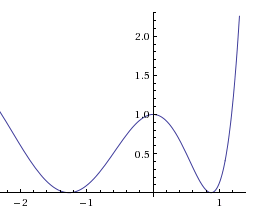
\includegraphics[width=\linewidth]{wells.png}
  \end{minipage}
  \begin{minipage}[r]{0.65\linewidth}
    What can be said if $h$ is minimal on non-degenerate critical
    points?
    
    \uncover<2->{
      \begin{thm}
        The eigenvectors of minimal eigenvalue concentrate only on
        ``minimal'' points. Eigenvectors and eigenvalues have an
        asymptotical expansion in powers of $N^{-\frac 12}$.
      \end{thm}
    }

    \uncover<3>{What is minimized ? The $\mu$ of the Hessian at this
      point.}
  \end{minipage}

  \vspace{2em}

\small{{\bfseries [9] Deleporte, A., Journal of Spectral Theory
    (accepted)}}
\end{frame}


\begin{frame}
\frametitle{Melin estimate}
\begin{itemize}
  \item Local result: for sections $u$ sufficiently concentrated around a
    minimal point of $f$ where the Hessian matrix is $q$, one has $\langle
    u,T_N(f)u\rangle \geq N^{-1}\mu(q)+CN^{-1-\epsilon}$.
  \uncover<2>{\item Global result: if $\mu_{inf}$ is the infimum of $\mu$ over all
    minimal points, then $$T_N(f)\geq N^{-1}\mu_{inf}+N^{-1-\epsilon}.$$}
  \end{itemize}

\small{
[8] Melin, A. Arkiv För Matematik 9, no. 1 (1971): 117–140}

\end{frame}

\begin{frame}
  \frametitle{Ideas for the proof}
  \begin{itemize}
  \item Local result: use the fact that the Szeg\H{o} kernel is
    equivalent to the $\C^n$ case near the diagonal, as $N\to
    +\infty$.
  \uncover<2>{\item Global result: pick a covering of the manifold with small open sets
    corresponding to the section, and ask
    that the section is relatively smaller at the intersection of the
    open sets than elsewhere.}
  \end{itemize}
\end{frame}

\subsection{Localization of the ground state}
\begin{frame}
  \frametitle{A general localization result}
  \begin{prop}
    Let $f\in C^{\infty}(M,\R)$ with $\min(f)=0$.
    Then any sequence $(u_N)$ of normalized eigenstates of $T_N(f)$
    with eigenvalues $O(N^{-\epsilon})$ is such that
$$\int_{\{f(x)\geq N^{-1+\delta}\}}|u_N(x)|^2 \dd Vol=O(N^{-\infty}).$$
  \end{prop}

  \uncover<2->{Indeed, the first eigenvalue is $O(N^{-1})$, so that $\langle
  u_N,fu_N\rangle=O(N^{-1})$.}

\uncover<3>{By induction, $\langle u_N,f^ku_N\rangle = O(N^{-k})$,
  hence the claim.}
\vspace{2em}

\small{{\bfseries [9] Deleporte, A., Journal of Spectral Theory
    (accepted)}}
\end{frame}

\begin{frame}
\frametitle{Subprincipal effects on localization}
  \begin{thm}
    Let $f\in C^{\infty}(M,\R)$ with $\min(f)=0$. Let $V$ at positive
    distance from $\{\mu=\mu_{min}\}$.
    Then, with $(u_N)$ as previously one has $$\int_{V}|u_N|^2\dd Vol=O(N^{-\infty}).$$
  \end{thm}
\uncover<2>{The proof uses the Melin estimates.}
\vspace{2em}

\small{{\bfseries [9] Deleporte, A., Journal of Spectral Theory
    (accepted)}\\{\bfseries [10] Deleporte, A., Arxiv preprint}.}
\end{frame}
\begin{frame}
  \frametitle{Expansions in the regular case}
  The regular case is a generalization of Helffer-Sj\"ostrand's
  ``miniwells''.
If $\mu$ is only minimal at one point $x_0$ near which $\{f=0\}$ is
    an isotropic submanifold, and the minimum is non-degenerate, then
    \begin{itemize}
    \item The first eigenvalue is simple and admits an expansion in
      powers of $N^{-\frac 14}$.
    \item The first eigenvector concentrates at speed $N^{-\frac 14+}$ on $x_0$ along
      $\{f=0\}$.
    \item Spectral gap $CN^{-\frac 32}$.
    \end{itemize}

\small{[11] Helffer, B., Sjöstrand, J. Current Topics in PDEs, 1986, 133–186\\{\bfseries [10] Deleporte, A., Arxiv preprint}.}
\end{frame}

\begin{frame}
  \frametitle{Crossing points}
  We treat the case where $\{f=0\}$ is a union of two sumbanifolds
  with a ``crossing point'', where $\mu$ is minimal.

  Toy model: $h(q_1,q_2,p_1,p_2)=p_1^2+p_2^2+q_1^2q_2^2$.
  
    \begin{itemize}
    \item The first eigenvalue is simple and admits an expansion in
      powers of $N^{-\frac 16}$.
    \item The first eigenvector concentrates  at speed $N^{-\frac 13+}$ on $x_0$ along
      $\{f=0\}$.
    \item Spectral gap $CN^{-\frac 43}$.
    \end{itemize}
    \vspace{2em}
    
\small{{\bfseries [10] Deleporte, A., Arxiv preprint}.}
\end{frame}

\begin{frame}
  \frametitle{Tools for the two cases}
  We constructed symplectic normal forms, which are new even in the
  context of pseudodifferential calculus.
\uncover<2->{  \begin{prop}
If $\sigma:U\to V$ is a local symplectomorphism between two K\"ahler
manifolds $M$ and $N$, then there is a sequence of maps
$\mathfrak{S}_N:M\to N$, such that, when acting on sequences of
sections microlocalising on $U$, 

\begin{itemize}
\item $\mathfrak{S}_N$ is an isometry modulo $O(N^{-\infty})$ error.
\uncover<3->{\item $\mathfrak{S}_NT_N(h)\mathfrak{S}_N^{-1}=T_N(\sigma\circ h + N^{-1}g_1+N^{-2}g_2+\cdots).$}
\end{itemize}
\end{prop}}

\uncover<4>{At the minimal points, the subprincipal symbol is
  prescribed by the Melin estimates on both sides.}
\end{frame}
\subsection{Future work}
\begin{frame}
  \frametitle{Perspective}
  \begin{enumerate}
  \item Work in progress:
    \begin{itemize}
    \item Exponential estimates in the analytic case,
      \uncover<2->{Tunnelling}
    \uncover<3->{\item Low-energy time evolution}
    \end{itemize}
  \item Conjectures:
    \begin{itemize}
    \uncover<4->{\item Where is $\mu$ minimal for the Kagome lattice?}
    \uncover<5>{\item The Scottish flag: $T_N(\cos(q)+i\cos(p))$ on the two-torus.}
    \end{itemize}
  \end{enumerate}
\end{frame}

\end{document}
%%% Local Variables:
%%% mode: latex
%%% TeX-master: t
%%% End:
